\newpage
\subsection{\particle}
\secwriter{A. Zupanc}

\paragraph{General overview}

This class is a common representation of all particle types, e.g.:
\begin{itemize}
 \item final state particles (FS particles)
 \begin{itemize}
  \item charged kaons, pions, electrons, muons, and protons reconstructed as {\tt Track}
  \item photons reconstructed as {\tt ECLGamma}
  \item long lived neutral kaons reconstructed in KLM
 \end{itemize}
 \item composite particles
 \begin{itemize}
  \item neutral pion pre-reconstructed as {\tt ECLPi0} 
  \item vee particles (short lived neutral kaon, $\Lambda$ baryon, converted photon) pre-reconstructed as {\tt MdstVee}\footnote{Note: 
  {\tt MdstVee} or equivalent data-object does not exist yet.}
 \item particles reconstructed by the user (via combinations)
 \end{itemize}
\end{itemize}

Private members are limited to those which completely define the particle and that are common to all particle types. Information which
exists and is unique only to a specific type of particles should not be saved inside the \particle class. Such information should be 
saved inside a specially designed data object which can be created and filled with some analysis module. This data object can be
related to the \particle objects of a specific type using BASF2 \relation. An example of such additional information and corresponding
data object are particle identification likelihoods which are stored in \pidLikelihood class. 

Private members are divided into persistent and transient data members. The former are those which can't be (easily) reproduced and therefore need
to be saved to \mudst while the latter can be easily reproduced (recalculated) on-demand.

\subsubsection{Data members}

The main and the most important data members of \particle class are the physics (kinematic) quantities:
\begin{itemize}
 \item 4-momentum vector and the point in which the momentum is estimated 
 \item the momentum-position error matrix (including the correlations between momentum and position estimates)
\end{itemize}
which enable reconstruction of unstable particles and determination of their decay (and production) vertices, etc... All other data members
are included in principle to make analyses user friendly, faster, ...

\paragraph{Persistent members} 
\begin{itemize}
 \item {\color{blue}energy in LAB} \hfill{float}
 \item {\color{blue}momentum vector in LAB} \hfill{$3\times$float}
 \begin{itemize}
  \item the point in which the momentum vector is estimated is given in the position/decay vertex data member
 \end{itemize}
 \item {\color{blue}position/decay vertex} \hfill{$3\times$float}
 \begin{itemize}
  \item in the case of charged FS particles this is point-of-closest-approach (POCA), which is copied from the \track data object.
  \item in the case of neutrals ($\gamma$, $\pi^0$, or $K^0_L$) this is the point of origin which is assumed during the 
  reconstruction of these particles (e.g. point $(0,0,0)$ or IP). This point is  copied from the corresponding \mdst data object. 
  \item in the case of composite particles this is the decay vertex determined by some vertexing module and until then this point is (0,0,0)
 \end{itemize}
 \item {\color{blue}$7\times7$ error matrix} \hfill{$28\times$float}
 \begin{itemize}
  \item order of elements in the error matrix is: $p_x, p_y, p_z, E, x, y, z$
  \item in the case of (pre-reconstructed) FS particles the error matrix is filled in \particle constructor
  \item in the case of composite particles the error matrix is filled when a kinematic fit is performed (until then is empty)
  \item internally the error matrix is saved as one dimensional array with 28 elements 
 \end{itemize}
 \item {\color{blue}$\chi^2$ probability of the fit} \hfill{float}
 \begin{itemize}
  \item in case of charged FS particles a $\chi^2$ value of the track fit is stored and in case of all composite particles the 
  $\chi^2$ value of the kinematic fit is stored (e.g. mass-constrained, vertex, mass-constrained vertex fit)
  \item variable is initialized to -1
  \begin{itemize}
   \item $\chi^2<0$ indicates that the error matrix is not valid
   \item $\chi^2\geq 0$ indicates that the error matrix is valid
  \end{itemize}
 \end{itemize}
 \item {\color{blue}number of degrees of freedom of the fit} \hfill{unsigned}
 \begin{itemize}
  \item same as above
 \end{itemize}
 \item {\color{blue} PDG code} \hfill{int}
 \begin{itemize}
  \item identification code of a particle
  \item PDG code is also used as a proxy to nominal values of different physics quantities (like nominal mass, lifetime, ...)
 \end{itemize}
 \item {\color{blue} vector of {\tt StoreArray$\langle$Particle$\rangle$} indices of daughter particles} \hfill{vector$\langle$unsigned$\rangle$}
 \begin{itemize}
  \item As it will be discussed later all \particle objects are stored inside the same StoreArray$\langle$Particle$\rangle$. This vector
  thus holds indices of daughter particles within this StoreArray$\langle$Particle$\rangle$.
 \end{itemize}
 \item {\color{blue} mdst index of an object from which the FS particle is created} \hfill{unsigned}
 \begin{itemize}
  \item only filled for (pre-reconstructed) particles
  \item needed in order to check for overlaps when performing combinations
 \end{itemize}
 \item {\color{blue} type of the \mdst object from which the particle is created } \hfill{int}
 \begin{itemize}
  \item see {\tt EParticleType} enum
  \item motivation is the same as above
 \end{itemize}
 \item {\color{blue}flavor type} \hfill{unsigned}
 \begin{itemize}
  \item in order to support automatic reconstruction of charged conjugated decays
 \end{itemize}
 \item {\color{blue}decay mode identifier} \hfill{unsigned}
 \begin{itemize}
  \item user specified code that uniquely identifies the decay mode in which this particle is reconstructed
 \end{itemize}
\end{itemize}

\paragraph{Transient members}

\begin{itemize}
 \item {\color{blue} pointer to the {\tt StoreArray$\langle$Particle$\rangle$}}\hfill{\tt TClonesArray$\ast$}
 \begin{itemize}
  \item  {\tt StoreArray$\langle$Particle$\rangle$} in which this \particle object is saved
 \end{itemize}
\end{itemize}

\subsubsection{Enums}

\begin{itemize}
 \item {\color{blue}\tt EParticleType}
 \begin{itemize}
  \item {\tt\color{red} c\_Undefined}: \particle is created by user from 4-momentum; has no daughters or BASF2 relation to any \mdst dataobject
  \item {\tt\color{red} c\_Track}: \particle is created from reconstructed \track \mdst dataobject; has BASF2 relation to \track
  \item {\tt\color{red} c\_ECLGamma}: \particle is created from reconstructed {\tt ECLGamma} \mdst dataobject; has BASF2 relation to {\tt ECLGamma}
  \item {\tt\color{red} c\_Pi0}: \particle is created from reconstructed {\tt ECLPi0} \mdst dataobject; has BASF2 relation to {\tt ECLPi0}; internally stores indices of two daughter \particle
  \item {\tt\color{red} c\_KLong}: \particle is created from reconstructed {\tt ECLPi0} \mdst dataobject
  \item {\tt\color{red} c\_MCParticle}: \particle is created from {\tt MCParticle} \mdst dataobject;
  \item {\tt\color{red} c\_Composite}: \particle is reconstructed by the user; internally stores indices to daughter \particle
 \end{itemize}
\end{itemize}

\subsubsection{Constructors}

\paragraph{Constructors from \mdst dataobjects}
\begin{itemize}
 \item the \particle constructor from the following \mdst data objects are provided: {\tt \track, ECLGamma, ECLPi0, MDSTVee, MDSTKlong(?)} and {\tt MCParticle}
 \item the \particle data members are initialized/set within these constructors to the values given in the table below
\end{itemize}
\begin{center}
 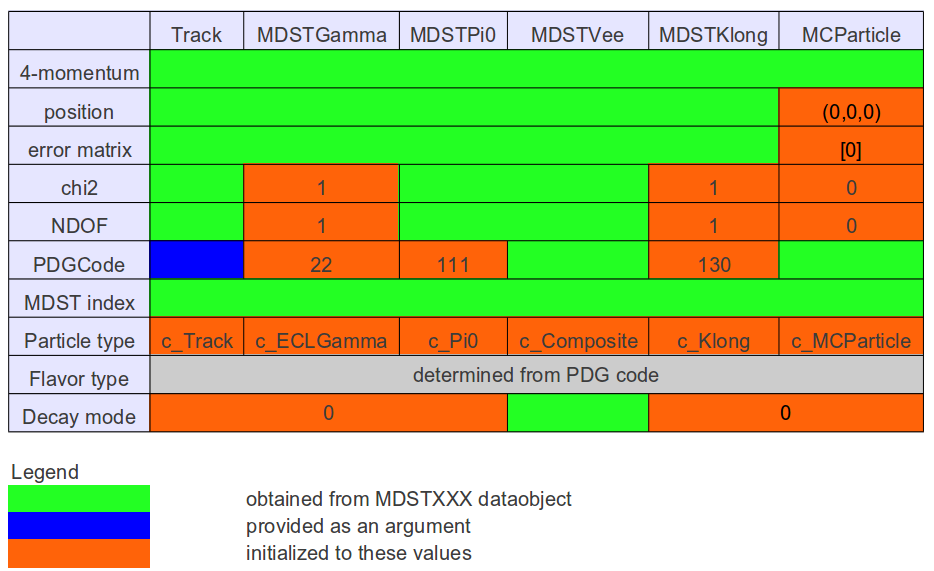
\includegraphics[width=0.9\textwidth]{DataModel/figs/particleConstructorsFromMDST.png}
\end{center}

\paragraph{Other constructors}
\begin{itemize}
 \item {\bluett Particle(TLorentzVector momentum, int pdgCode)}
 \begin{itemize}
  \item the simplest constructor
  \item all other members are set to their default values (0)
  \item {\tt particleType} member is set to {\tt c\_Undefined}
 \end{itemize}
 \item {\footnotesize\bluett Particle(TLorentzVector mom, int pdgCode, unsigned flavorType, vector$\langle$unsigned$\rangle$ daugIndices)}
 \begin{itemize}
  \item constructor for composite particles
  \item {\tt particleType} member is set to {\tt c\_Composite}
 \end{itemize}
\end{itemize}


\subsubsection{Member functions}

\paragraph{Getters/Setters for private members}

The table given below provides list of available getters and setters for private members:
\begin{center}
 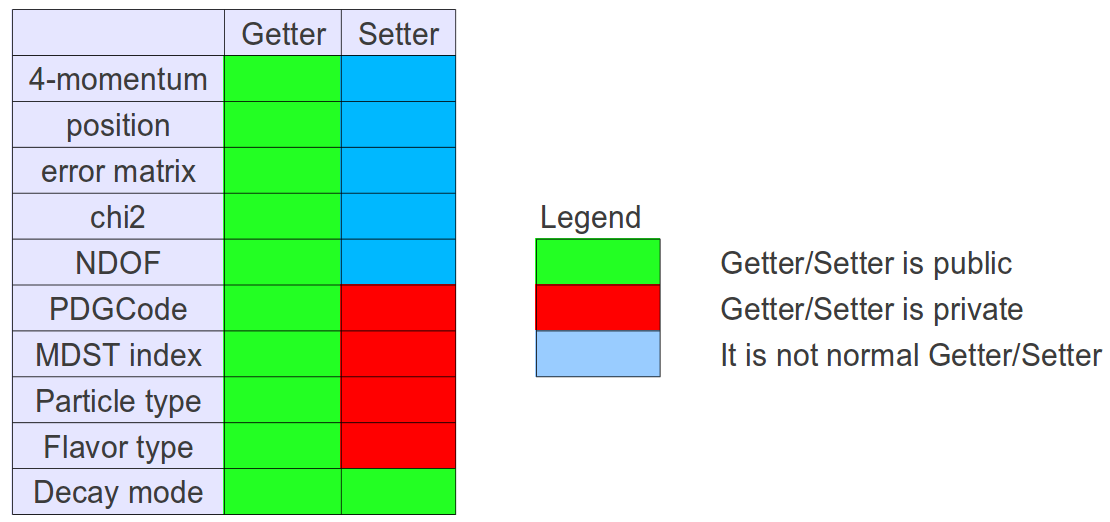
\includegraphics[width=0.9\textwidth]{DataModel/figs/particleGetterSetter.png}
\end{center}
The getters for kinematic quantities return momentum, position and error matrix as {\tt TLorentzVector, TVector3}, and {\tt TMatrixFSym}, 
respectively. In addition, a function that returns the position (or decay vertex) as the \vertex object is provided.

Special care needs to be taken when it comes to setters for these kinematic quantities, since it can lead to inconsistent 
state, if they are allowed to be modified individually. The momentum and position (decay vertex)
can be correlated and can be thus modified only at once and should not be allowed to be modified individually. 
This means that are no standard setters for these three quantities, like {\tt setMomentum(TLorentzVector), setVertex(TVector3)}, and 
{\tt setErrorMatrix(TMatrixFSym)}, but instead only single public function is provided which enables updating of kinematic quantities
and $\chi^2$ and number of degrees of freedom members:
\begin{itemize}
 \item {\bluett updateMomentum(TLorentzVector, TVector3, TMatrixFSym, float, unsiged)}
\end{itemize}

\paragraph{Additional accessors to other frequently used kinematic quantities}

\begin{itemize}
  \item {\bluett float getP()/getMomentumMagnitude()} -- magnitude of momentum in LAB
  \item {\bluett float getPx()/getPy()/getPz()} -- $x/y/z$ component of momentum in LAB
  \item {\bluett float getMass()} -- invariant mass
  \item {\bluett float getMassError()} -- estimated invariant mass uncertainty
  \item {\bluett float getX()/getY()/getZ()} -- $x/y/z$ component of position (decay vertex)
  \item {\bluett TMatrixFSym getMomentumErrorMatrix()}  -- $4\times4$ momentum error submatrix
  \item {\bluett TMatrixFSym getVertexErrorMatrix()}  -- $3\times3$ momentum error sub-matrix
  \item {\bluett float getMassBeforeKinematicFit()} -- returns the invariant mass before any kinematic fit is performed (with or without mass constraint)
  \begin{itemize}
   \item a transient transient data member can be added (set in the constructor for composite \particle)
   \item or (re-)calculated on demand from original 4-momenta of FS particles (which are never overwritten)
   \item {\bf this should be utility function, since it is needed only during writing out to Ntuple}
  \end{itemize}
  \item {\bluett float getCharge()} -- returns the reconstructed charge 
  \begin{itemize}
   \item determined by summing over the charges of daughter particles
   \item if \particle has no daughter particles then the nominal charge based on its PDG code is returned
  \end{itemize}
\end{itemize}

\paragraph{Additional accessors to nominal quantities} All functions that return nominal values have to start with {\tt getPDG...()} These 
quantities are accessed via {\tt TDatabasePDG}.
\begin{itemize}
 \item {\bluett getPDGCode()} -- returns PDG code
 \item {\bluett getPDGMass()} -- returns nominal mass
 \item {\bluett getPDGWidth()} -- returns intrinsic width
 \item {\bluett getPDGLifetime()} -- returns lifetime
 \item {\bluett getPDGCharge()} -- returns nominal charge
\end{itemize}

\paragraph{Accessors/modifiers of daughters}

\begin{itemize}
 \item {\bluett appendDaughter(Particle)} -- appends (index) of provided \particle to the vector of daughter indices (sets {\tt ParticleType} to {\tt c\_Composite})
 \item {\bluett appendDaughter(int)} -- appends provided index to the vector of daughter indices (sets {\tt ParticleType} to {\tt c\_Composite})
 \item {\bluett unsigned getNDaughters()} -- returns the number of daughters
 \item {\bluett Particle* getDaughter(int)} -- returns the pointer to i-th daughter
 \item {\bluett vector$\langle$Particle*$\rangle$ getDaughters()} -- returns the vector of pointers to all daughters
 \item {\bluett vector$\langle$int$\rangle$ getDaughterIndices()} -- returns the vector of daughter indices
 \item {\bluett vector$\langle$Particle*$\rangle$ getFinalStateDaughters()} -- returns the vector of pointers to FS particle daughters
\end{itemize}

In addition the function that checks whether or not {\tt this} \particle shares any of the FS particles with \particle given as an argument:
\begin{itemize}
 \item {\bluett bool overlapsWith(Particle*)}
\end{itemize}
